
\begin{figure}
	\centering
	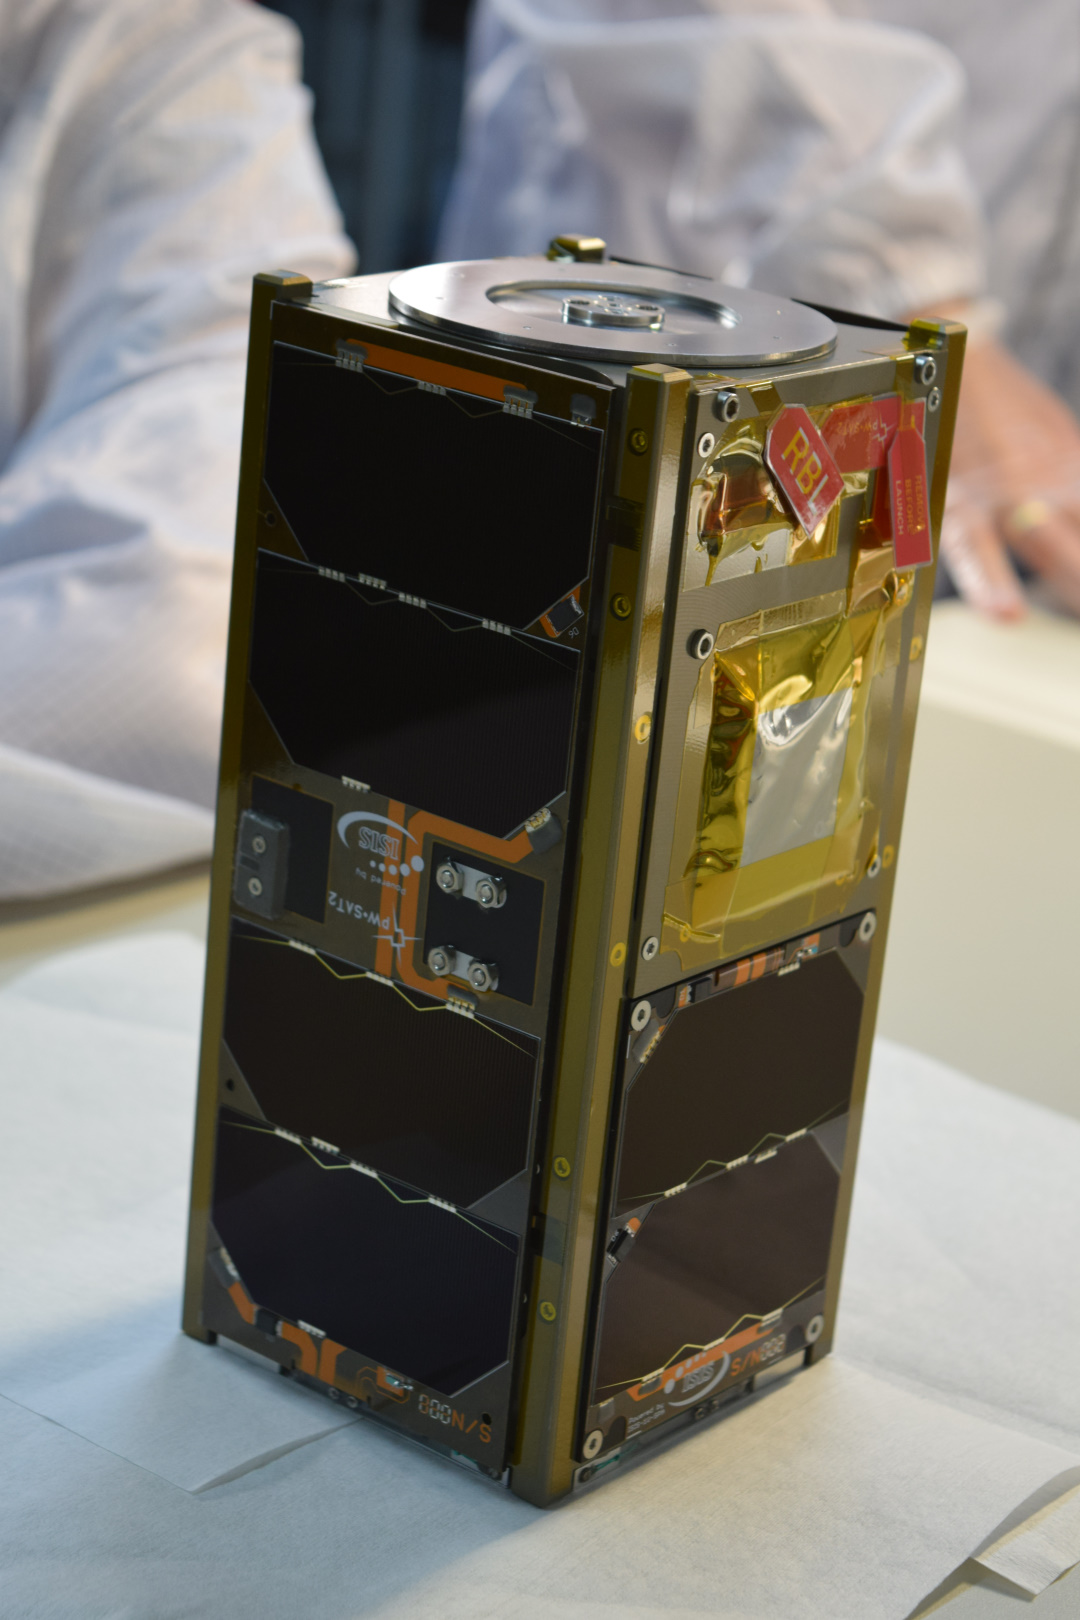
\includegraphics[width=0.5\textwidth]{img/pw-sat.jpg}
	\caption{\label{fig:basic:pw-sat} PW-Sat2 before launch}
\end{figure}

\section{PW-Sat2 Basic information}



\begin{itemize}
 \item 2U CubeSat.
 \item International designator: \textbf{18099BJ}, NORAD Catalog Number: \textbf{43814}
 \item Launched 3rd December 2018 from Vandenberg Air Force Base onboard Falcon 9.
 \item Mission main objective: test deorbitation sail.
 \item Mission secondary objectives: test experimental sunsensor, measure radiation doze using RadFET, test solar array deployments system.
 \item Orbit:
 \begin{itemize}
	\item SSO: started at 590 km, decaying about 80 meters per day (about 560 km after 1 year).
	\item About 6 communication windows every day on our latitude. 
	\item No orientation control (only detumbling available). Because of the spinning and opened sail the communication is often "one-way".	
 \end{itemize}
 \item Radio (using amateur bands):
 \begin{itemize}         
	\item Uplink: 145.900, AFSK, 1200bps, AX.25
    \item Downlink: 435.275, BPSK, 9600bps, AX.25
    \item Full-duplex communication possible.
 \end{itemize}
\end{itemize}